\documentclass[draft]{beamer}
\usepackage{beamerthemesplit} % kam neu dazu
\usepackage[utf8]{inputenc}
\usepackage[T1]{fontenc}
\usepackage[ngerman]{babel}



\begin{document}
\title{Mößbauereffekt} 
\author{Paul Kremser, Tobias Grussenemyer}
\date{Versuchsdurchführung: 1. bis 12. März 2010} 

\frame{\titlepage} 

\frame{\frametitle{Inhaltsverzeichnis}\tableofcontents} 

\section{Einleitung}
\subsection{Historisches}
\subsection{Anwendungen}

\frame{\frametitle{Rudolf Mößbauer}
Er ging davon aus, dass sich zwei Quanten die auf diese Weise wechselwirken mit der doppelten Rückstoßgeschwindigkeit aufeinander zu bewegen müssten.
Diese Theorie folgt direkt aus der Impulserhaltung und schien zunächst auch durch das Experiment bestätigt zu werden. Zuerst untersuchte Mössbauer nämlich die
Resonanzabsorption bei Zimmertemperatur und darüber. Als er aber begann Quelle und Absorber abzukühlen, stieg die Intensität des Messsignals plötzlich steil an,
und zwar über die bei hohen Temperaturen gemessene.
}

\section{Theorie und Aufbau}
\subsection{Emission und Absorption}
\begin{enumerate}
 \item Geht ein 
 \item Energieeichung des MCA mit Hilfe eines Americium Strahlers und verschiedener metallischer Floureszenzplättchen (Aufbau mit Drehscheibe)
 \item Mit dem SCA ein Fenster auf die 14,4 KeV Linie setzen.
 \item Mit Hilfe verschiedener Aluminiumplättchen sollen Untergrundmessungen bei verschiedenen Dicken gemacht werden um später auf die Dicke Null extrapolieren zu können.
 \item Aufnahme der Spektren des Einlinien- (Eisen) Absorbers und des 6-Linien- (Edelstahl) Absorbers.
\end{enumerate}
\subsection{Hyperfeinstruktur}

\subsection{Rückstoßfreie Resonanzabsorbtion}

\subsection{Aufbau}


\frame{\frametitle{Resonanzabsorption}
\begin{itemize}
 \item Beim Kernübergang von angeregtem- in Grundzustand
 \item wird ein Photon erzeugt $E_\gamma \approx E_a - E_g$
 \item dieses kann einen anderen Kern anregen
 \item Resonanzabsorption: Gleiche angeregte Zustände
 \item Aus der Impulserhaltung folgt ein Engergiefehlbetrag der doppelten Rückstoßenergie
\end{itemize}
}

\frame{\frametitle{Energieverschiebung}
\begin{figure}
 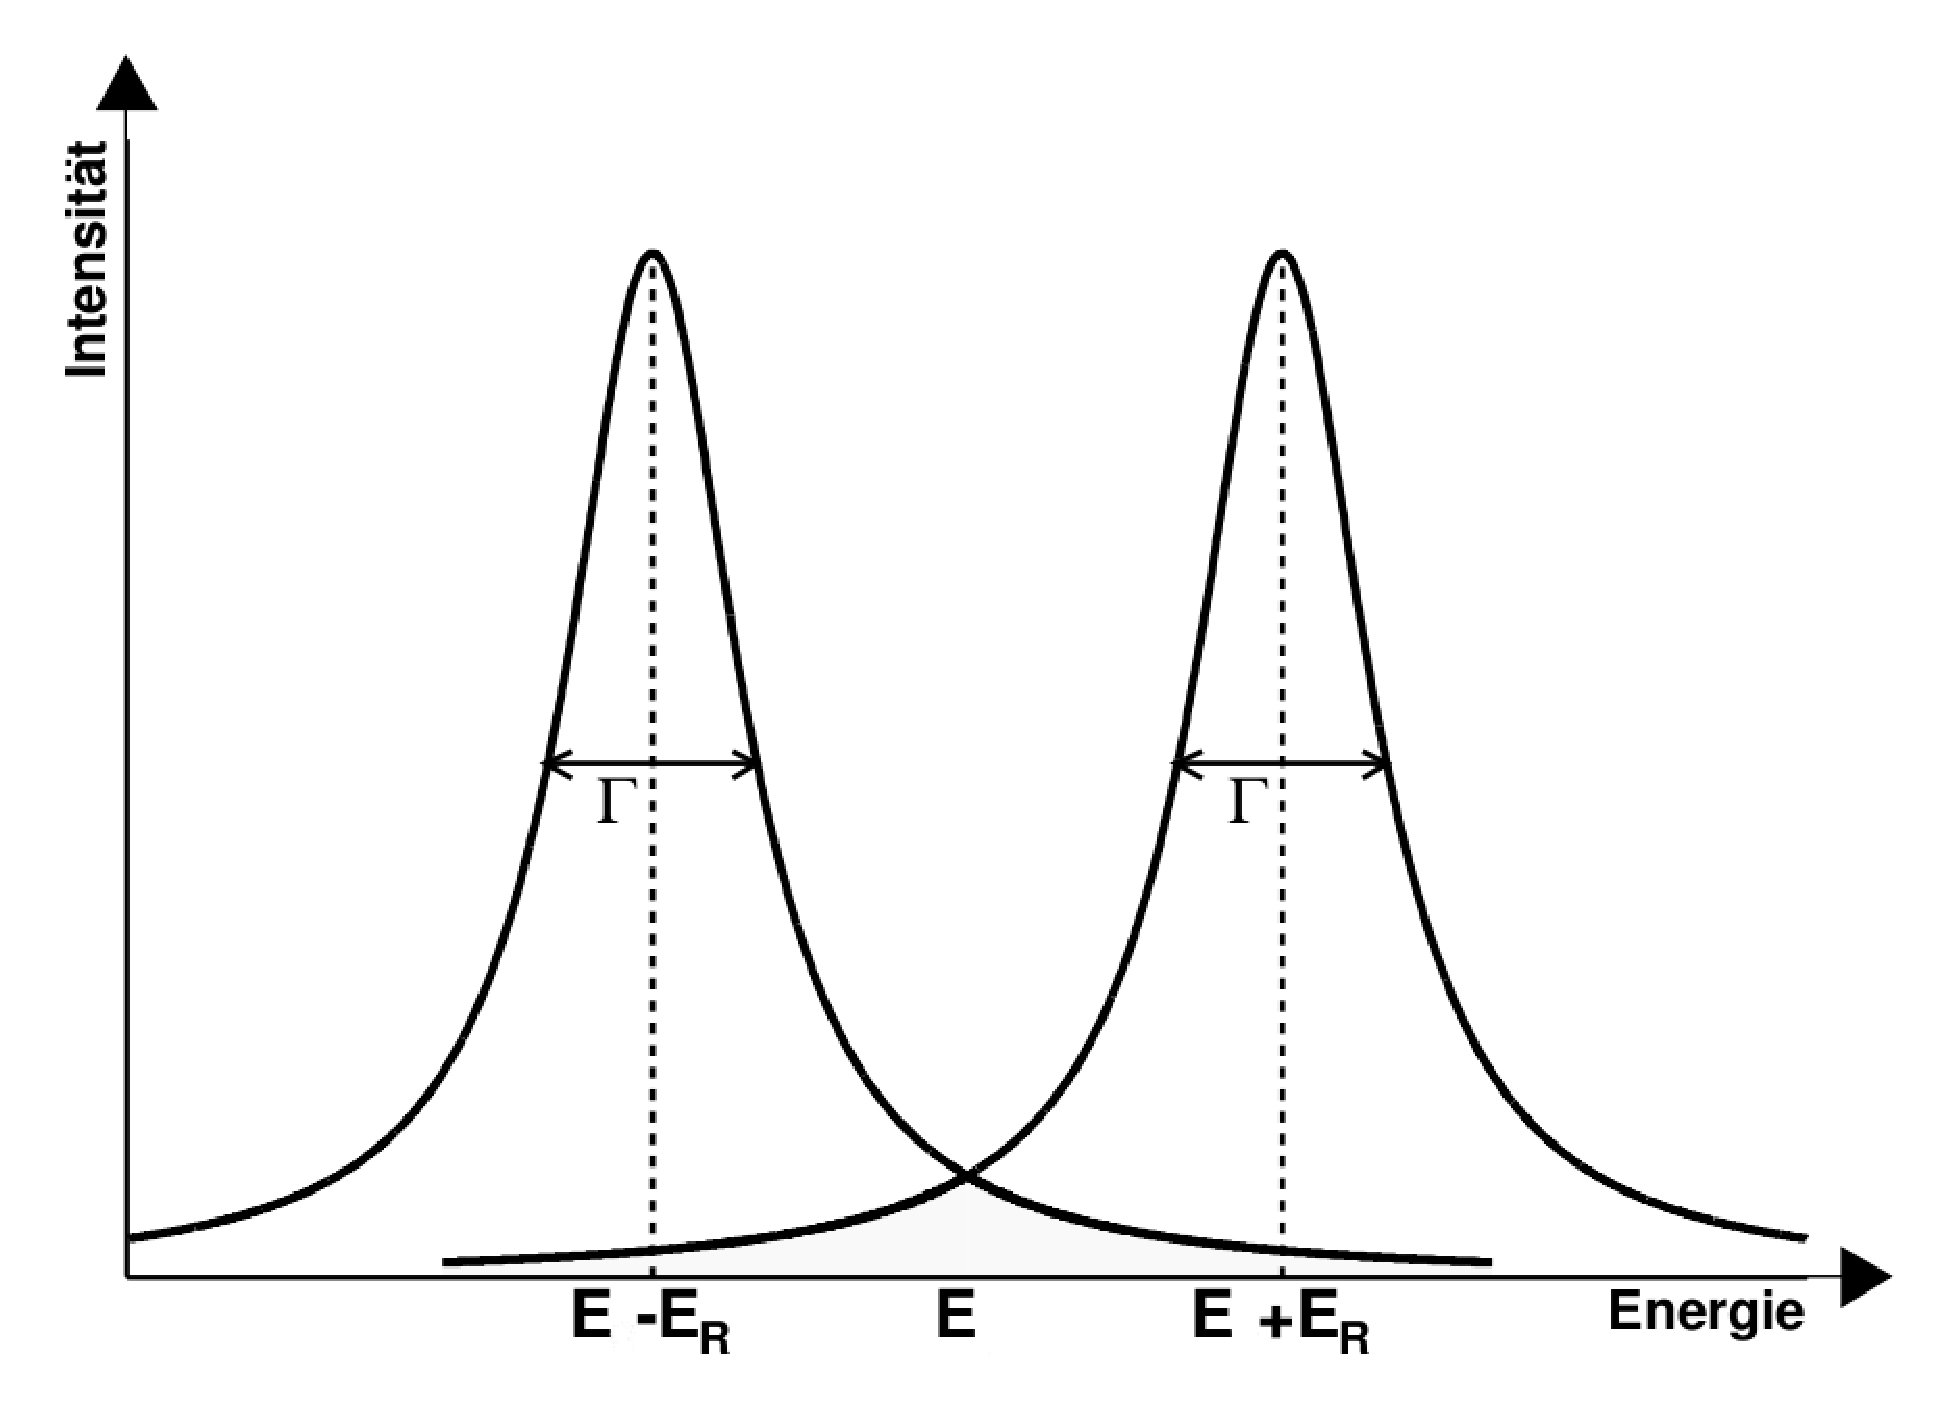
\includegraphics[width=0.7\linewidth]{pictures/energieverschiebung.eps}
 \caption{Energieverschiebung von Emissions- und Absorptionslinie}
 \label{energieverschiebung}
\end{figure}
}

\frame{\frametitle{Debye-Waller-Faktor}
Wie schon erwähnt kann es aber auch vorkommen, dass keine rückstoßfreie Resonanzabsorption auftritt da bei der Absorption oder Emission Gitterschwingungen (Phononen) 
angeregt werden können und somit dem Photon doch wieder nicht die volle Energie des Übergangs zur Verfügung steht. Der Debye-Waller-Faktor $f$ gibt an wie viel rückstoßfreie Resonanzabsorption
auftritt. Er hängt von der Temperatur und der Übergangsenergie ab:
}
\frame{\frametitle{Debye-Waller-Faktor}
\begin{align}
 f = exp\left[ -\frac{3E_R}{2k_B\Theta}\left(1+\left(\frac{2T}{\Theta}\right)^2 \int\limits_{0}^{\frac{\Theta}{T}} \frac{x~dx}{e^x - 1}\right)\right]
\end{align}
und lässt sich für kleine Temperaturen $(T<<\Theta)$ und Kerne im arteigenen kubischen Gitter annähern durch:
\begin{align}
 f \approx exp \left[ -\frac{E_R}{k_B\Theta}\left(\frac{3}{2} + \left(\frac{\pi T}{\Theta}\right)^2\right)\right]
\end{align}
wobei $T$ die absolute Temperatur, $k_B$ die Boltzmannkonstante, $E_R$ die Rückstoßenergie und $\Theta$ die Debye-Temperatur ist.
}

\section{Durchführung und Ergebnisse}
\subsection{Aufgabenstellung}
\frame{\frametitle{Aufgabenstellung}
\begin{enumerate}
 \item Energieeichung des MCA
 \item Energiefenster auf 14,4 KeV Linie
 \item Untergrundmessung
 \item Spektrum des 1-Linien- (Eisen) Absorbers
 \begin{itemize}
  \item Isomerieverschiebung
  \item Effektive Absorberdicke, Wirkungsquerschnitt, Debye-Waller-Faktor
  \item Linienbreite und Lebensdauer
 \end{itemize}
 \item Spektrum des 6-Linien- (Edelstahl) Absorbers.
 \begin{itemize}
  \item Isomerieverschiebung
  \item Kernmagnetisches Moment
  \item Magnetfeld am Kernort
 \end{itemize}
\end{enumerate}
}

\subsection{Energieeichug und Energiefenster}
\frame{\frametitle{Energieeichung}
\begin{block}{Wofür Energieeichung}
 Zur Identifikation des 14,4$keV$ Peaks im Spektrum \\
 $\Rightarrow$ Beziehung zwischen Kanal des MCA und Energie 
\end{block}
\begin{block}{Wie}
 Americium-Quelle mit verschiedenen Metallplättchen \\
 $\Rightarrow$ Bekannte Energien mit identifizierbaren Peaks
\end{block}
\vfill
\begin{tabular}{|l|l|l|l|l|l|}
\hline
Stoff & Rubidium & Molibdän & Silber & Terbium & Barium\\
Energie $K_{\alpha}$/keV & 13.3 & 17.44 & 22.1 & 44.23 & 32.06 \\
\hline
\end{tabular}

}
\frame{\frametitle{Gaußfits an $K_\alpha$-Linien}
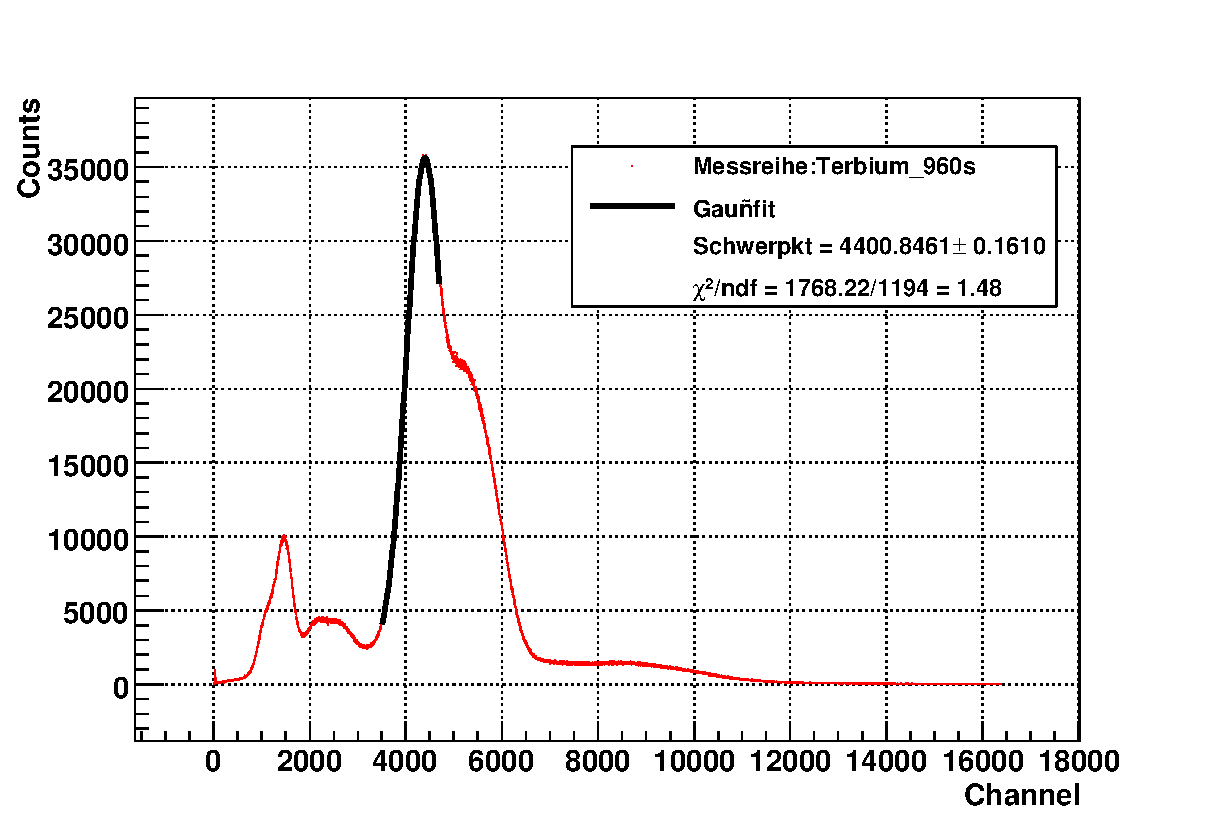
\includegraphics[width=0.9\linewidth]{pictures/eichung_terbium.eps}
}
\frame{\frametitle{Gaußfits an $K_\alpha$-Linien}
\begin{columns}
        \column{.5\textwidth}
                 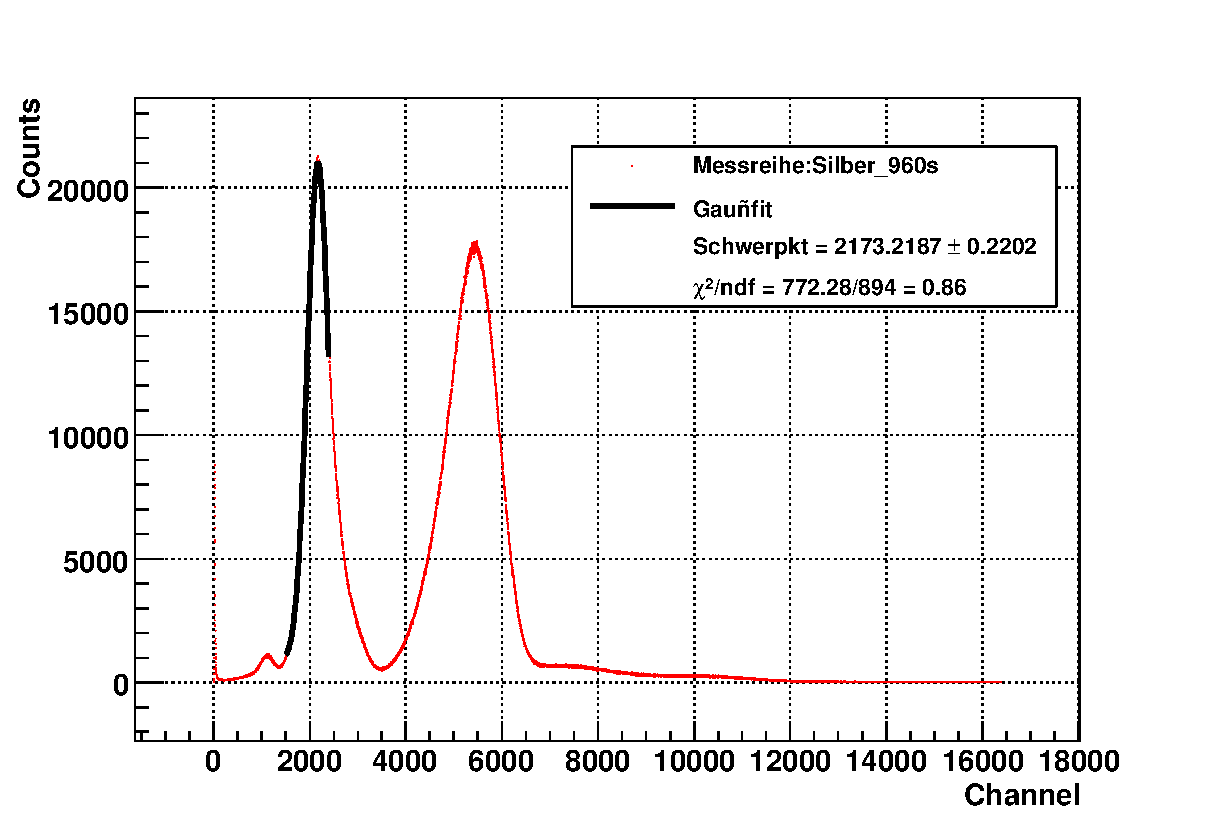
\includegraphics[width=0.9\linewidth]{pictures/eichung_silber.eps}
        \column{.5\textwidth}
		 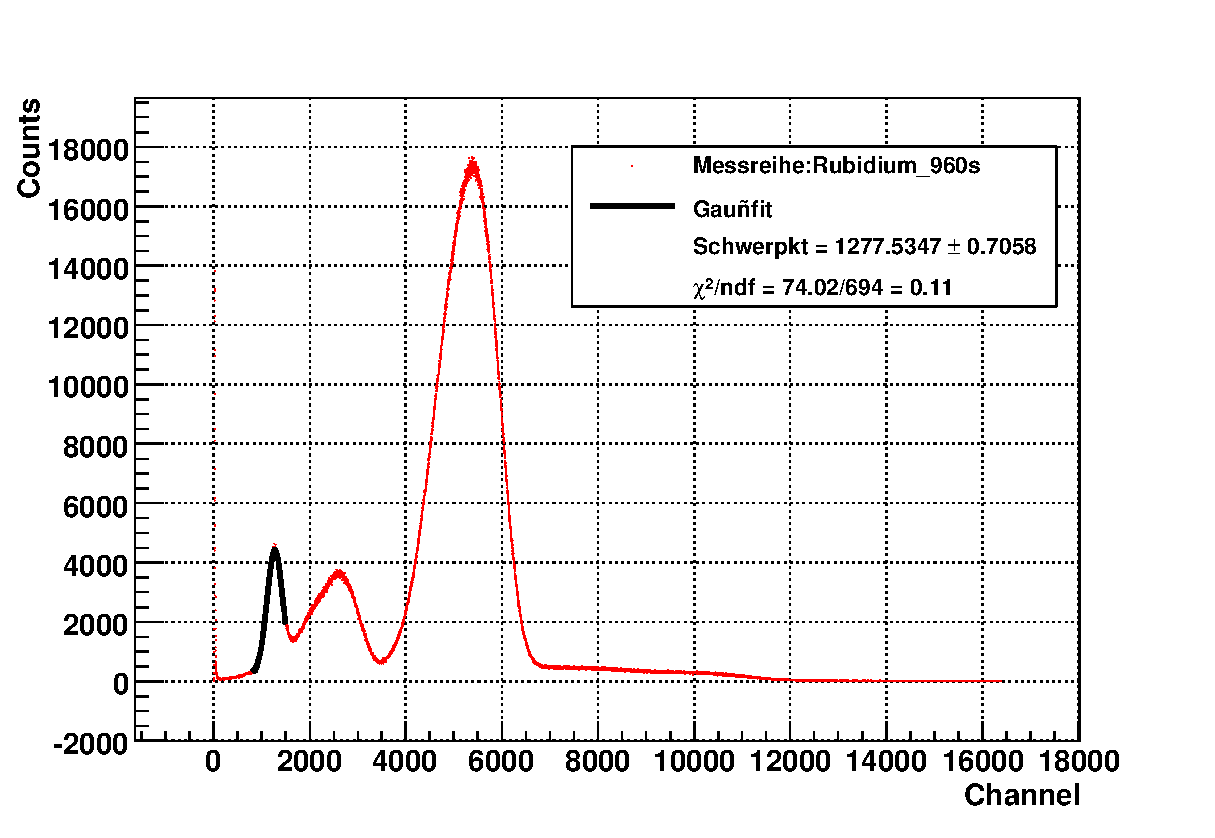
\includegraphics[width=0.9\linewidth]{pictures/eichung_rubidium.eps}
\end{columns}
\begin{columns}
        \column{.5\textwidth}
                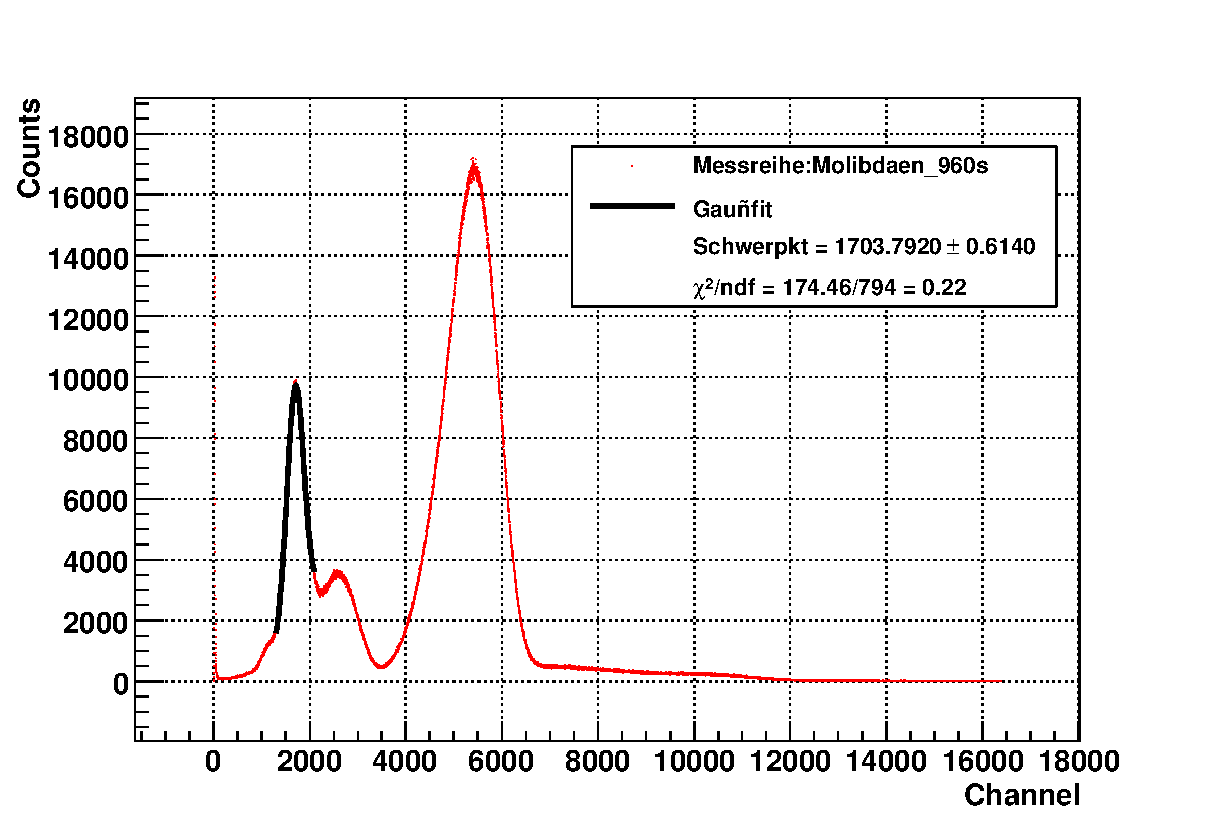
\includegraphics[width=0.9\linewidth]{pictures/eichung_molibdaen.eps}
        \column{.5\textwidth}
                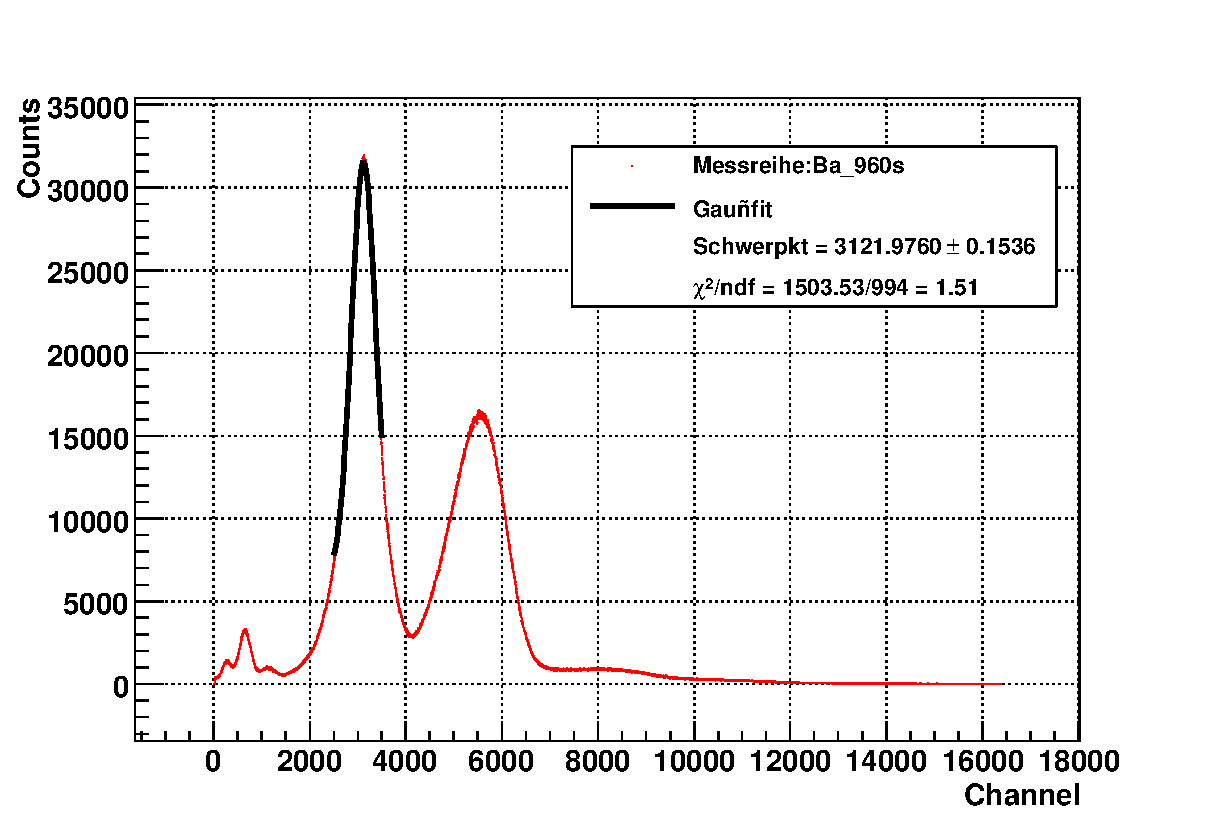
\includegraphics[width=0.9\linewidth]{pictures/eichung_barium.eps}
\end{columns}
}
\frame{\frametitle{Fit an die Orte der Gaußkurven}
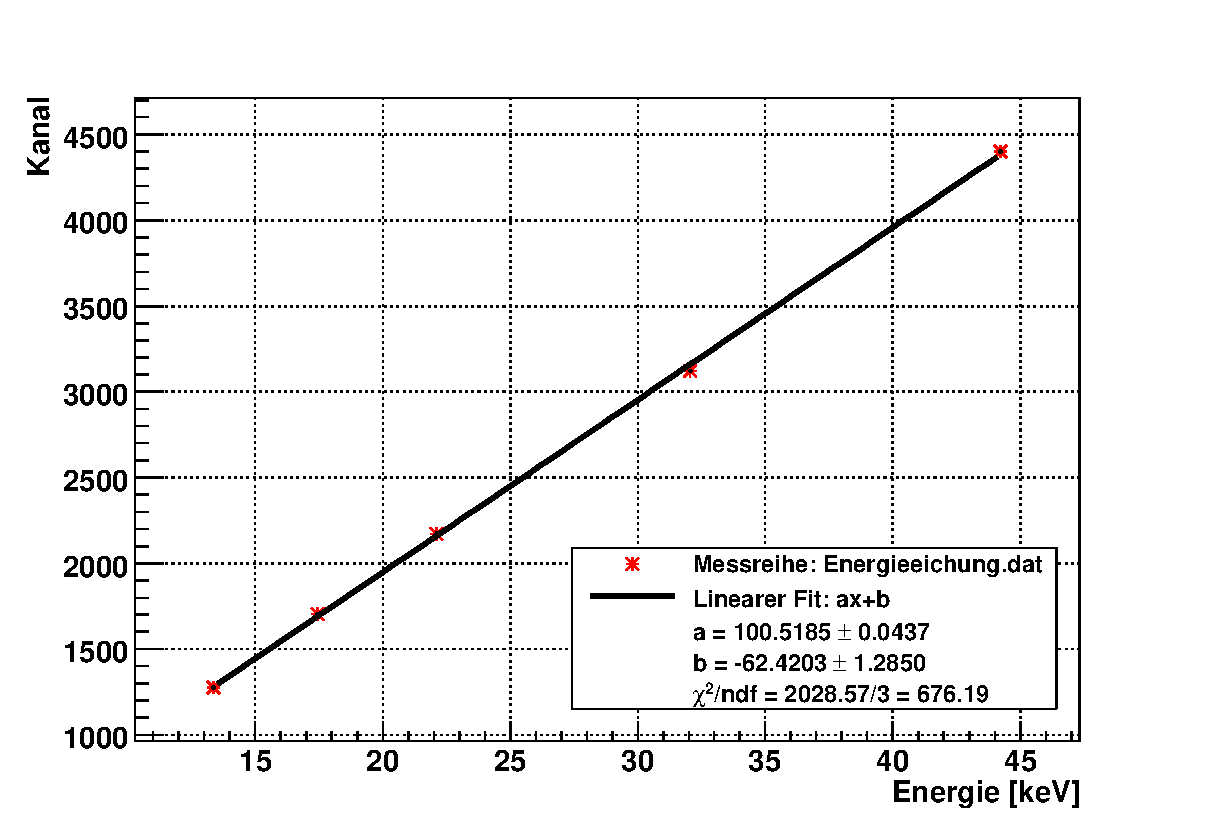
\includegraphics[width=0.9\linewidth]{pictures/eichung_linear.eps}
}
\frame{\frametitle{Fit an die Orte der Gaußkurven}
\begin{block}{Fit}
\begin{align*}
  C = a \cdot E + b \hspace{30pt}
\end{align*}
\begin{align*}
 \textnormal{mit}\hspace{30pt}a = 100.52 \pm 0.04\textnormal{ und }b =  -62.42 \pm 1.285
\end{align*}
\end{block}

\begin{block}{14,4 keV Linie}
\begin{align*}
  C_{14.4keV} = 1385,07 \pm 1,27
\end{align*}
\end{block}
}
\frame{\frametitle{Fenstereinstellung}
\begin{block}{Warum ein Fenster verwenden}
 Mößbauermessung geschieht mit Zähler, getriggert durch Motor \\
 $\Rightarrow$ Nur Ereignisse mit 14,4 keV sollen gezählt werden
\end{block}
\begin{block}{Single-Channel-Analyser}
 Einstellung: Unter- und Obergrenze für Energie \\
 Visualisierung über MCA
\end{block}
}
\subsection{Untergrund}
\frame{\frametitle{Untergrund}
\begin{block}{Compton-Streuung}
\begin{itemize}
 \item Quelle hat im wesentlichen zwei Peaks ($14,4 keV$ und $122 keV$)
 \item Comptonstreuung erzeugt Untergrund im Messfenster
 \item Nur indirekt messbar
\end{itemize}
\end{block}
\begin{block}{Abschirmung durch Aluminium}
Bei zunehmender Dicke erwartet man unterschiedliche Abschwächung der beiden Energien \\
$\Rightarrow$ Doppelter Expotentialfit und Extrapolation auf Dicke 0
\end{block}
}
\frame{\frametitle{Untergrundfit}
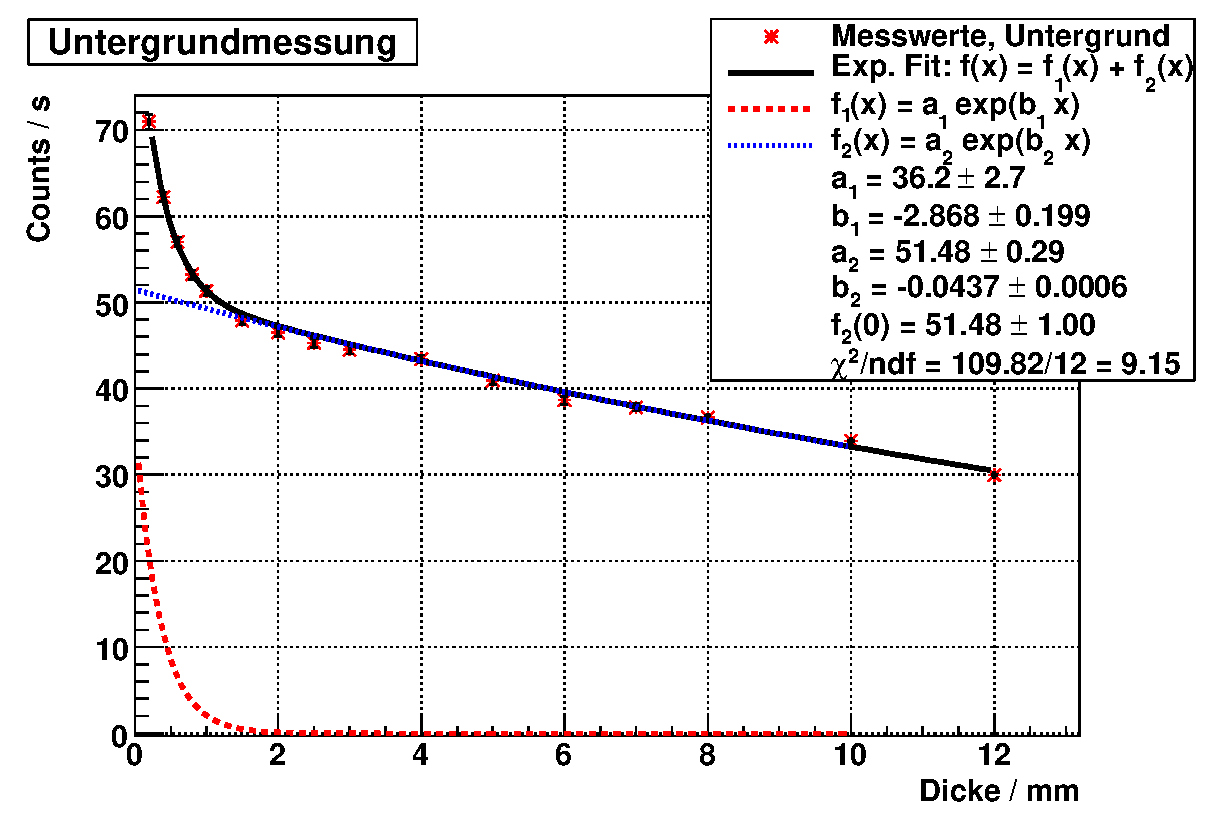
\includegraphics[width=0.9\linewidth]{pictures/untergrund.eps}
}
\frame{\frametitle{Untergrundfit}
\begin{block}{Fit}
\begin{align*}
  f_2 (d) = (50,38 \pm 0,78) \cdot exp (-0,0413 \pm 0,0027) \frac{Counts}{s}
\end{align*}
\end{block}

\begin{block}{Untergrundzählrate}
\begin{align*}
  R_{Untergrund} = (50,38 \pm 0,78) \frac{Counts}{s} 
\end{align*}
\end{block}
}
\subsection{Die Messung}
\frame{\frametitle{Absorberschlitten und Motor}

}
% 1 Linien (Edelstahl)
\frame{\frametitle{Edelstahl-(1-Linien-)absorber}

}

% 6 Linien (Eisen)

\subsection{Ergebnisse}
\section{Die Entdeckung der Langsamkeit}
\end{document}

